\documentclass[tikz,border=10pt]{standalone}
\usetikzlibrary{calc, intersections, angles, quotes}

\begin{document}
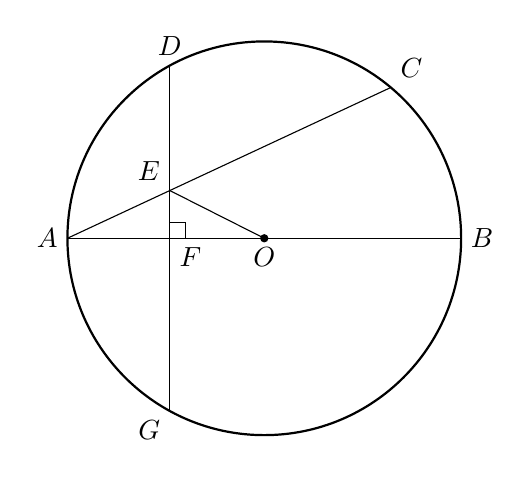
\begin{tikzpicture}
    % 定义参数
    \def\R{2.5}  % 圆的半径
    
    % 定义坐标
    \coordinate (O) at (0,0);
    \coordinate (A) at (-\R, 0);
    \coordinate (B) at (\R, 0);
    
    % 画圆
    \draw[thick] (O) circle (\R);
    
    % 确定点 C (大致在右上角圆弧上)
    \coordinate (C) at (50:\R);
    
    % 确定竖直弦 DG (位置坐标 F 设在圆心左侧)
    \def\xpos{-1.2}
    \coordinate (F) at (\xpos, 0);
    
    % 计算 D 和 G (利用勾股定理确定圆上点，y^2 = R^2 - x^2)
    \pgfmathsetmacro{\ypos}{sqrt(\R*\R - \xpos*\xpos)}
    \coordinate (D) at (\xpos, \ypos);
    \coordinate (G) at (\xpos, -\ypos);
    
    % 计算 E (线段 AC 与 DG 的交点)
    \path[name path=AC] (A) -- (C);
    \path[name path=DG] (D) -- (G);
    \path [name intersections={of=AC and DG, by=E}];
    
    % 绘制线段
    \draw (A) -- (B);
    \draw (A) -- (C);
    \draw (D) -- (G);
    \draw (E) -- (O);
    
    % 绘制直角标记
    \draw (\xpos, 0.2) -- (\xpos+0.2, 0.2) -- (\xpos+0.2, 0);
    
    % 标注点
    \fill (O) circle (1.5pt) node[below] {$O$};
    \node[left] at (A) {$A$};
    \node[right] at (B) {$B$};
    \node[above] at (D) {$D$};
    \node[below left] at (G) {$G$};
    \node[above right] at (C) {$C$};
    \node[above left] at (E) {$E$};
    \node[below right] at (F) {$F$};
    
\end{tikzpicture}
\end{document}